\documentclass{article}
%\title{ \LARGE \textsc{Digital Communication Report on} \\ \textsc{\Huge Channel Polarization} }
%\author{\textbf{By: Himanshu Sharma [1610110149]} \\\\ \textit{Under the supervision of Prof. Vijay K. Chakka} \\\\\\ \huge Dept. of Electrical Engineering \\\\\\\\ \huge Shiv Nadar University\\
%NH91, Tehsil Dadri, Greater Noida, Uttar Pradesh 201314}
\title{\textsc{Channel Polarization}}
\newcommand\tab[1][1cm]{\hspace*{#1}}
\author{\textbf{By: Himanshu Sharma}  \tab[6cm] \textbf{Roll No.: 1610110149}}
\date{}

\usepackage[margin=1.1in]{geometry}
\usepackage{float}
\usepackage{graphicx}
\usepackage{amsmath}

\begin{document}
\maketitle
Channel polarization is a process in which $N$ channels are generated from $N$ independent copies of a B-DMC $W$. The newly generated channel is $\{W_{N}^{(i)}: 1 \leq i \leq N \}$. As $N \rightarrow \infty$, the symmetric capacity $I(W_{N}^{(i)})$ either becomes 0 or it becomes 1 for all vanishing fractions of $i$. Note that the symmetric capacity of a B-DMC $W$ is given by
\begin{equation}
I(W) = \sum_{x \in X}\sum_{y \in Y}\frac{1}{2}W(y|x)\log_{2}\frac{W(y|x)}{0.5W(y|0) + 0.5W(y|1)}
\end{equation}
\section{Channel Combining}
Channel combining is a phase operation used in channel polarization wherein \textbf{copies} of B-DMC $W$ are combined in a recursive manner to produce a vector channel $W_{N}: X^{N} \rightarrow Y^{N}$. The value of $N$ is $2^{n}$ where $n \geq 0$. That means, the very first copy of the channel $W_{1}=W$, because $n=0$ for $N=1$. Similarly, $W_{2}: X^{2} \rightarrow Y^{2}$.
\par The transition probability is given by $W_{2}(y_{1}, y_{2}|x_{1}, x_{2})$, note the $W_{2}$, its not $W$. Asking for the value $W_{2}(y_{1}, y_{2}|x_{1}, x_{2})$ is same as asking $W(y_{1}|x_{1})W(y_{2}|x_{2})$, becuase sending $u_{1}$ and $u_{2}$ in channel $W_{2}$ is same as sending $x_{1}$ and $x_{2}$ in two copies of channel $W$ separately. That means,
\begin{center}
$W_{2}(y_{1}, y_{2}|x_{1}, x_{2}) = W(y_{1}|x_{1})W(y_{2}|x_{2}) = W(y_{1}|u_{1}\oplus u_{2})W(y_{2}|u_{2})$ because $x_{1} = u_{1} \oplus u_{2}$.
\end{center}
\begin{figure}[H]
\centering
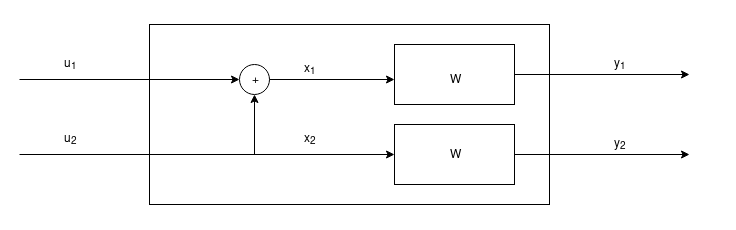
\includegraphics[width=0.8\textwidth, height=0.2\textheight]{twochannel.png}
\caption{Channel $W_{2}$}
\end{figure}
The mapping between $u^{N}$ and $y^{N}$ is done by,
\begin{equation}
y_{i}^{N} = u_{i}^{N}G_{N} \textrm{ }\forall i \in \{1, ...., N\}
\end{equation}
Where
\[G_{2} = 
\begin{bmatrix}
1 & 0 \\
1 & 1
\end{bmatrix}
\]
Similarly, for $W_{4}$ also, the kernel matrix is $G_{4}$ where, 
\[G_{4} = 
\begin{bmatrix}
1 & 0 & 0 & 0 \\
1 & 0 & 1 & 0 \\
1 & 1 & 0 & 0 \\
1 & 1 & 1 & 1
\end{bmatrix}
\]
\begin{figure}[H]
\centering
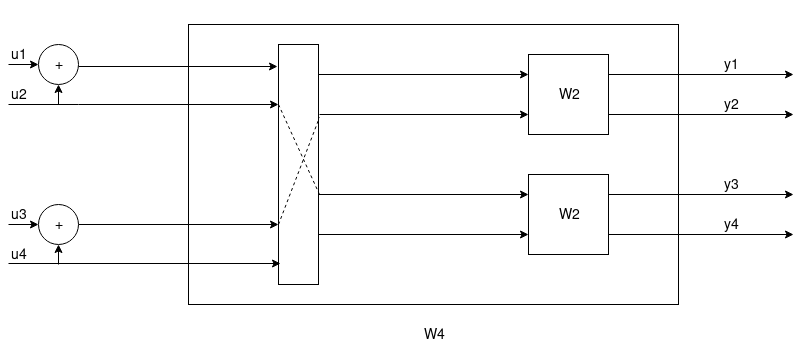
\includegraphics[width=0.8\textwidth, height=0.2\textheight]{w4.png}
\caption{Channel $W_{4}$}
\end{figure}
\begin{figure}[H]
\centering
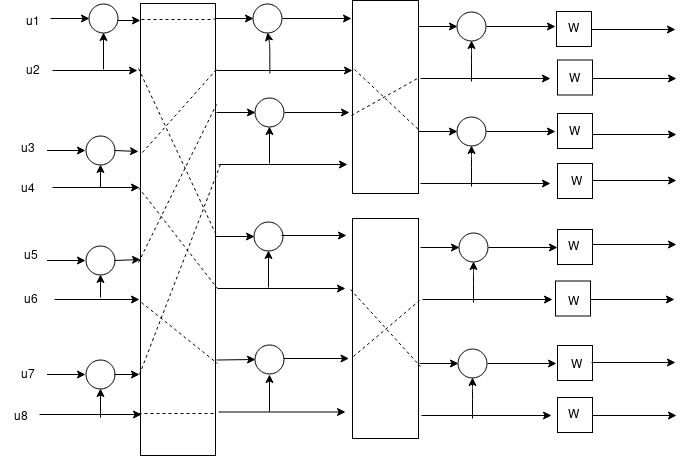
\includegraphics[width=0.8\textwidth, height=0.5\textheight]{w8.png}
\caption{Channel $W_{8}$}
\end{figure}
The vertical rectangular box shown in the channel $W_{4}$ is called the \textbf{reverse shuffle operator} which takes odd indices at one side and even on the other. If one carefully goes through both $W_{4}$ and $W_{2}$, then the outputs $[y_{1}, y_{2},y_{3},y_{4}]$ are $[u_{1}\oplus u_{2} \oplus u_{3} \oplus u_{4}, u_{3} \oplus u_{4}, u_{2} \oplus u_{4}, u_{4}]$. The same can be obtained from the kernel matrix $G_{4}$.
\[
\begin{bmatrix}
u_{1} & u_{2} &u_{3}&u_{4}
\end{bmatrix}
\begin{bmatrix}
1 & 0 & 0 & 0 \\
1 & 0 & 1 & 0 \\
1 & 1 & 0 & 0 \\
1 & 1 & 1 & 1
\end{bmatrix}
=
\begin{bmatrix}
u_{1}\oplus u_{2} \oplus u_{3} \oplus u_{4} & u_{3} \oplus u_{4} &  u_{2} \oplus u_{4} & u_{4}
\end{bmatrix}
\] 

\section{Channel Polarization}
Channel polarization is a process in which a B-DMC $W$ gives rise to $N$ channels such that $W_{N}^{(i)} \textrm{ } \forall  i \in [1, N]$. In this process, the generated channels either go to zero information state or pure information state of $I(W) = 1/0$ as $N \rightarrow \infty$. The following diagram shows the polarization effect. 
\begin{figure}[H]
\centering
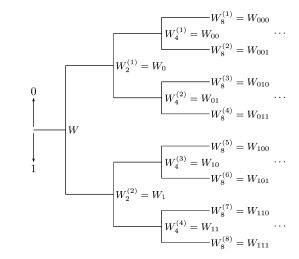
\includegraphics[width=0.4\textwidth, height=0.2\textheight]{chpol.png}
\caption{Channel Polarization Effect}
\end{figure}
Considering the channel $W_{2}$, we can see that it has two copies of the original channel $W$ and therefore, it has a capacity of $2I(W)$ where $I(W) = 1 - f(p)$ is the Shannon's capacity for a BEC and $p$ denotes the transition probability of the BEC.
\subsection{Single Step Transform}
Consider figure 1 again. This time, refer to the below shown diagram also, taken from the reference. 
\begin{figure}[H]
\centering
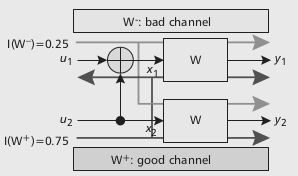
\includegraphics[width=0.4\textwidth, height=0.2\textheight]{w2polar.png}
\caption{Polarized Channel [1]}
\end{figure}
By applying the chain rule of the mutual information, this channel $W_{2}$ can be decomposed into two BEC with capacities $I(W^{-})$ and $I(W^{+})$ where $I(W^{-}) + I(W^{+}) = 2I(W)$. Also, note the following identities,
\begin{equation}
I(W^{-}) = I(W)^{2}
\end{equation}
and 
\begin{equation}
I(W^{+}) = 2I(W) - I(W)^{2}
\end{equation}
In the figure shown above, $I(W)=0.5$. This proves that the bad channel $W^{-}$ has a smaller capacity than the given BEC $W$, whereas the good channel $W^{+}$ has a larger capacity, that is, $I(W^{-} ) \leq I(W) \leq I(W^{+})$. 
\par Let us take over with the same case of $I(W)=0.5$, for BEC $W$. When this channel is polarized once, then $I(W^{-}) = 0.25$ and $I(W^{+}) = 0.75$. Consider `+' to be equivalent of 0 and `-' to be equivalent of 1, then the next will be of order 00, 01, 10, 11, i.e., ++, +-, -+ and --, with following values,
\begin{center}
$I(W^{++}) = 2I(W^{+}) - I(W^{+})^{2} = 0.9375$ \\
$I(W^{+-}) = I(W^{+})^{2} = 0.5625$ \\
$I(W^{-+}) = 2I(W^{-}) - I(W^{-})^{2} = 0.4375$ \\
$I(W^{--}) = I(W^{-})^{2} = 0.0625$ 
\end{center}

As we can see, the more we polarize, the more good and bad channels are generated with their respective channel capacities.
\subsection{The Matthew Effect}
The Matthew Effect is the summary of channel polarization. It says that as the length of the codeword goes to infinity, the capacity of the most good channel tends to one. The below plot shows the Matthew effect.
\begin{figure}[H]
\centering
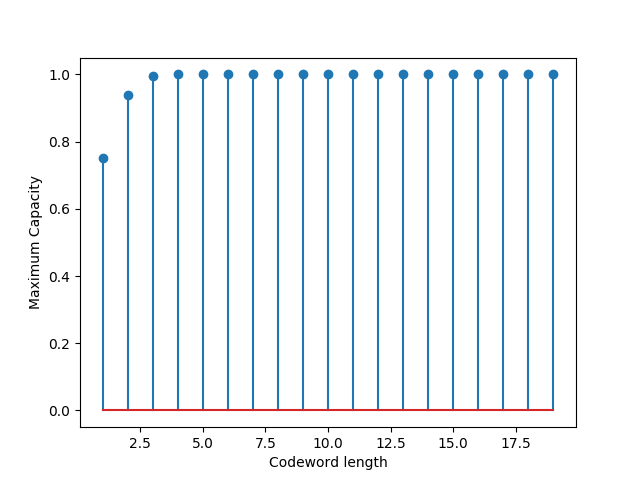
\includegraphics[width=0.8\textwidth, height=0.4\textheight]{matthew.png}
\caption{The Matthew Effect}
\end{figure}
Clearly, as the length of the codeword reaches 3, the capacity of the \textit{good} channel tends to 1. That is, the more codeword length you have, the better will be the capacity of the good channel. Hence, we find that the capacities of most of the polarized channels tend to either 1 (good channels with little noise) or 0 (bad channels with full noise). Equivalently, the error probabilities of the noiseless channels or noisy channels go to 0 or 1. Consider yet another plots for Matthew effect.

\begin{figure}[H]
\centering
\begin{minipage}{0.49\textwidth}
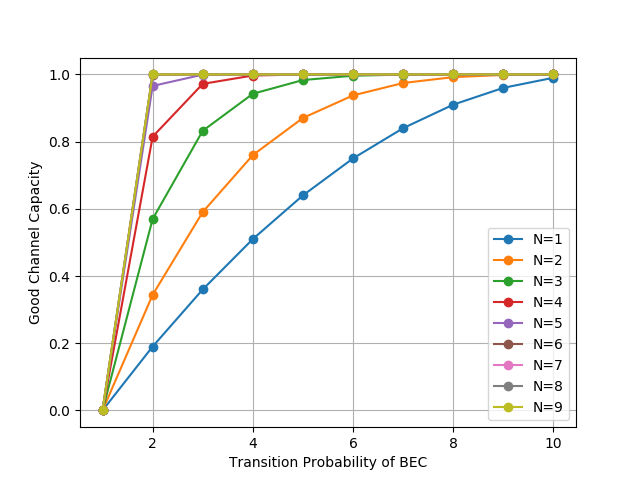
\includegraphics[width=\linewidth]{good_channels.png}
\caption{Good Channels for different levels}
\end{minipage}
\begin{minipage}{0.49\textwidth}
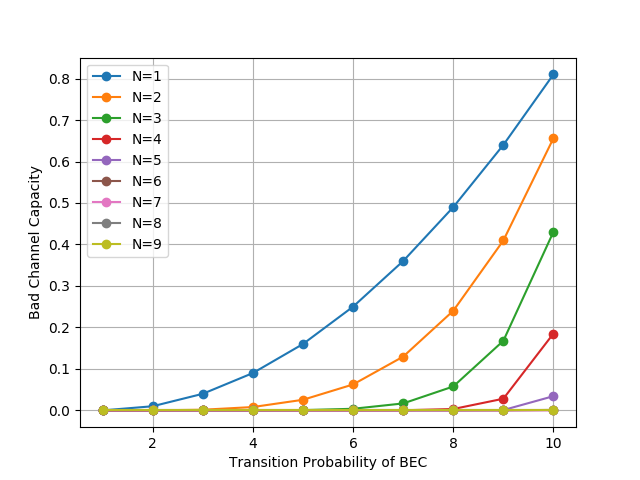
\includegraphics[width=\linewidth]{bad_channels.png}
\caption{Bad Channels for different levels}
\end{minipage}
\end{figure}
Clearly, the larger the $N$ we choose, more quickly the maximum capacity of 1 is achieved. But the case is opposite for bad channels. For bad channels, the lower $N$ you choose, you would be more better off. That is, in a hypothetical case, where we would like to use a noisy bad channel, then according to the figure 8, the best case would be to take the original single copy of the channel at a transitition probability of 0.9. And, for the good channel, we should use as much copies of the original B-DMC at any transition probability from 0.1 to 1.

\section{Channel Selection and the Reliability Sequence}
Till now, we saw that generating polar codes and polarizing a B-DMC is not a big deal at all. The twist comes when we have to decide what all channels to choose from a given polarized channels. This is given by the reliability sequence. Please refer to the Python codes in this report to know how reliability sequences are generated.
\end{document}